\documentclass{beamer}
\usepackage[ngerman]{babel}
\usepackage[utf8]{inputenc}
\usepackage{setspace} 
\usepackage{amsmath}
\usepackage{amsthm}
\usepackage{pgfplots}
\usepackage{siunitx}
\usepackage{caption}
\usepackage{graphicx}
\usepackage{eurosym}
\sisetup{locale = DE}
\sisetup{per-mode=fraction}
% Lade Beamer Stile
\usepackage{beamerthemesplit}
\usetheme{Rochester}
\usecolortheme{crane}
\setbeamercolor{bgcolor}{fg=black,bg=green!15!white}
\title{Übungsaufgabe Kleinspeicher}
\subtitle{Aufgabe 1}
\author{Heiko Schröter}
\date{\today}

\setbeamertemplate{enumerate item}{\alph{enumi})}
\newtheorem{satz}{Satz}

\begin{document}

\frame{\titlepage}

\frame{\tableofcontents}
\section{Aufgabe}
\section{Lösung}
\subsection{Aufgabe a)}
\subsection{Aufgabe b)}
\subsection{Aufgabe c)}

\frame
{
  \frametitle{Beschreibung}

 \begin{minipage}[t]{0.45\linewidth}
 \centering
 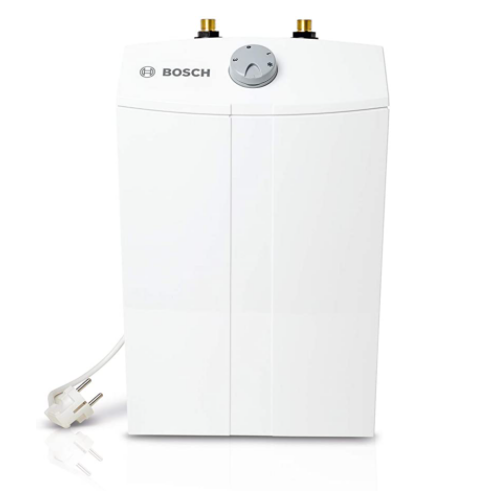
\includegraphics[width=.75\linewidth]{Kleinspeicher.png}
 \captionof{figure}{Kleinspeicher}
 \end{minipage}
 \hfill
 \begin{minipage}[t]{0.45\linewidth}
 \centering
 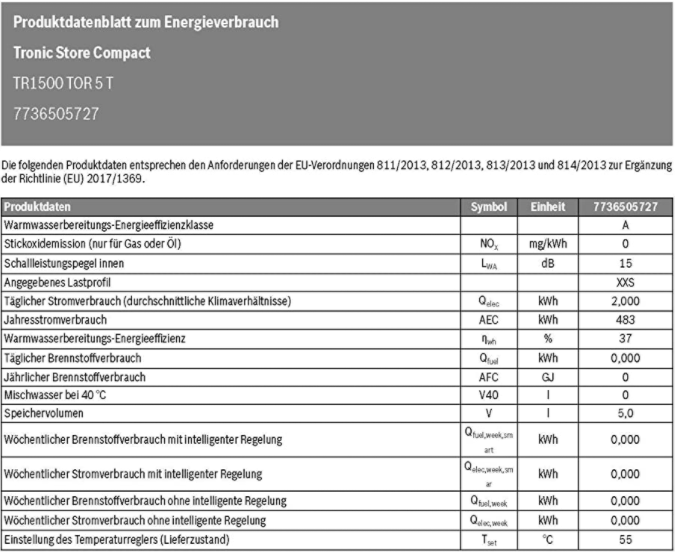
\includegraphics[width=1\linewidth]{Produktdatenblatt.png}
 \captionof{figure}{Produktdatenblatt}
 \end{minipage} 
}

\frame[allowframebreaks]
{
  \frametitle{Produktdatenblatt zum Energieverbrauch}
{{\footnotesize   Die folgenden Produktdaten entsprechen den Anforderungen der EU-Verordnungen 811/2013, 812/2013, 813/2013 und 814/2013 zur Ergänzung der Richtlinie(EU) 2017/1369.}
}\newpage
{
  \begin{scriptsize}
	\begin{tabular}{|p{6cm}|c|c|c|}
	\hline 
	\rule[-1ex]{0pt}{2.5ex} \textbf{Produktdaten} & \textbf{Symbol} & \textbf{Einheit} & \textbf{7736505727} \\ 
	\hline 
	\rule[-1ex]{0pt}{2.5ex} Warmwasserbereitungs- Energieeffizienzklasse &  &  & A \\ 
	\hline 
	\rule[-1ex]{0pt}{2.5ex} Stickoxidemmission (nur für Gas oder Öl) & $NO_x$ & $\si{\milli\gram\per\kilo\watt\per\hour}$ & 0 \\ 
	\hline 
	\rule[-1ex]{0pt}{2.5ex} Schallleistungspegel innen & $L_{WA}$ & $\si{dB}$ & $\num{15}$ \\ 
	\hline 
	\rule[-1ex]{0pt}{2.5ex} Angegebenes Lastprofil & & & XXS \\ 
	\hline 
	\rule[-1ex]{0pt}{2.5ex} täglicher Stromverbrauch (durchschnittliche Klimaverhältnisse) & $Q_{elec}$ & $\si{\kilo\watt\hour}$ & $\num{2.000}$ \\ 
	\hline 
	\rule[-1ex]{0pt}{2.5ex} Jahresstromverbrauch & AEC & $\si{\kilo\watt\hour}$ & $\num{483}$ \\ 
	\hline 
	\rule[-1ex]{0pt}{2.5ex} Warmwasserbereitungs-Energieeffizienz & $\eta_{wh}$ & $\%$ & $\num{37}$ \\ 
	\hline 
	\rule[-1ex]{0pt}{2.5ex} Täglicher Brennstoffverbrauch & $Q_{fuel}$ & $\si{\kilo\watt\hour}$ & $\num{0.000}$ \\ 
	\hline 
	\rule[-1ex]{0pt}{2.5ex} Jährlicher Brennstoffverbrauch & AFC & $\si{\giga\joule}$ & $\num{0}$ \\ 
	\hline 
	\rule[-1ex]{0pt}{2.5ex} Mischwasser bei $\SI{40}{\celsius}$ & V40 & $\si{\liter}$ & $\num{0}$ \\ 
	\hline 
	\rule[-1ex]{0pt}{2.5ex} Speichervolumen & V & $\si{\liter}$ & $\num{5.0}$ \\ 
	\hline 
	\rule[-1ex]{0pt}{2.5ex} Wöchentlicher Brennstoffverbrauch & $Q_{fuel-week}$ & $\si{\kilo\watt\hour}$ & $\num{0.000}$ \\ 
	\hline 
	\rule[-1ex]{0pt}{2.5ex} Wöchentlicher Stromverbrauch & $Q_{elec-week}$ & $\si{\kilo\watt\hour}$ & $\num{0.000}$ \\ 
	\hline 
	\rule[-1ex]{0pt}{2.5ex} Einstellung des Temperaturreglers (Lieferzustand) & $T_{set}$ & $\si{\celsius}$ & $\num{55}$ \\ 
	\hline 
	\end{tabular}
  \end{scriptsize}
  }
}

\frame
{
\frametitle{Beschreibung}
Zum Spülen von Geschirr möchtest du das Wasser eines voll gefüllten Kleinspeichers ($\SI{5}{\liter}$) von Zimmertemperatur auf ca. $\SI{60}{\celsius} $ erhitzen. Der Kleinspeicher hat eine Leistung von $\SI{2}{\kilo\watt}$.
\begin{enumerate}
\item Welche Wärmeenergie muss dem Wasser zugeführt werden?
\item Wie lange dauert der Vorgang?
\item Was kostet das Erhitzen des Wassers bei einem Kilowattstunden-preis von 28 Cent?
\end{enumerate}
}

\frame
{
  \frametitle{Lösung a)}
	\begin{exampleblock}{}
		\begin{equation}
			Q = c \cdot m \cdot \Delta T
		\end{equation}
	\end{exampleblock}
  \begin{align*}           
               \uncover<1->{&=\SI{4.19}{\kilo\joule\per\kilogram\per\kelvin}\cdot\SI{5}{\kilogram}\cdot\SI{40}{\kelvin}}\\
               \uncover<2->{&=\SI{838}{\kilo\joule}}\\
  \end{align*}
}

\frame
{
  \frametitle{Lösung b)}
	\begin{exampleblock}{}
		\begin{equation}
			P=\dfrac{Q}{t} \Rightarrow t=\dfrac{Q}{P}
		\end{equation}
	\end{exampleblock}
  \begin{align*}           
               \uncover<1->{&=\dfrac{\SI{838}{\kilo\watt\second}}{\SI{2}{\kilo\watt}}}\\
               \uncover<2->{&=\SI{419}{\second}\approx \SI{7}{\minute}}
  \end{align*}
}

\frame
{
  \frametitle{Lösung c)}
  \begin{equation*}
  \SI{838}{\kilo\joule}=\SI{838}{\kilo\watt\second}=\dfrac{838}{3600} \si{\kilo\watt\hour}\approx\SI{0.23}{\kilo\watt\hour}
  \end{equation*}
  \setstretch{1.5}
	$\SI{1}{\kilo\watt\hour}$ kostet $0.28$ \euro \\
	$\SI{0.23}{\kilo\watt\hour}$ kosten ca. $0.06$ \euro \\
  	Das Erwärmen des Wassers kostet ca. 6 Cent.
}
\end{document}